\documentclass{article}
\usepackage{asymptote}

\usepackage{amsmath, enumitem, graphicx, geometry}
\usepackage[inline]{asymptote}
\geometry{margin=1in}
\begin{asydef}
usepackage("bm");
texpreamble("\def\V#1{\bm{#1}}");
import geometry;
\end{asydef}

\begin{document}

\begin{center}
{\Large\bfseries Worksheet 11/6}\\[0.25cm]
{\large 6 November, 2025}\\[1cm]
\end{center}

\begin{enumerate}[itemsep=2.85cm]
    \item There are $81$ grid points (uniformly spaced) in the square shown in the diagram below, including the points on the edges. Point $P$ is in the center of the square. Given that point $Q$ is randomly chosen among the other $80$ points, what is the probability that the line $PQ$ is a line of symmetry for the square?
        \begin{figure}
            \centering
            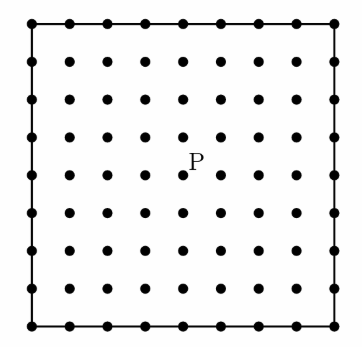
\includegraphics[width=0.5\linewidth]{image.png}
            \caption{For question 1}
            \label{fig:placeholder}
        \end{figure}
    \item Five different awards are to be given to three students. Each student will receive at least one award. In how many different ways can the awards be distributed? 
    \item How many integers between 1000 and 9999 have four distinct digits?
    \item In the small country of Mathland, all automobile license plates have four symbols. The second must be a vowel (A, E, I, O, or U), the first and third must be two different letters among the 21 non-vowels, and the fourth must be a digit (0 through 9). If the symbols are chosen at random subject to these conditions, what is the probability that the plate will read "SIX7"?
    \item A dessert chef prepares the dessert for every day of a week starting with Sunday. The dessert each day is either cake, pie, ice cream, or pudding. The same dessert may not be served two days in a row. There must be cake on Friday because of a birthday. How many different dessert menus for the week are possible?
    \item Marty has $24$ apples. In how many ways can he share them with Varun and Sreyas so that each of the three people has at least two apples?
\end{enumerate}
\end{document}